% !TEX root = ../dissertation.tex

\chapter{Mathematical Background}
This is some text
\section{Dumbbell Spacecraft Equations of Motion}\label{sec:dumbbell}

In this section we derive the equations of motion of a rigid spacecraft under the influence of the gravitational attraction of a homogenous asteroid.
The motion of a spacecraft around an asteroid is markedly different than that of Earth orbiting vehicles.
First, the gravitational field around an asteroid is highly irregular and complex. 
The usual assumption of a spherical potential is not valid for small or irregular shaped bodies.
Furthermore, since the magnitude of the gravitational attraction is relatively small, non-gravitational effects, such as solar radiation pressure or third-body effects, become much more significant.
As a result, the orbital environment is generally quite complex and it is difficult to generate analytical insights, such as the Keplerian two-body solution.

A second key consideration is the coupling between rotational and translational states around the asteroid.
The coupling is induced due to the different gravitational forces experienced on various parts of the spacecraft.
The effect of the gravitational coupling is related to the parameter \(\epsilon = \frac{r}{R_c}\), where \(r\) is the characteristic spacecraft length and \(R_c\) is the orbital radius~\cite{hughes2004}.
For Earth based missions, the orbital radius is several orders of magnitude larger than the spacecraft length and \(\epsilon\) is small.
As a result, the corresponding gravitational moment is weak and can be neglected. 
Therefore, the translational and rotational equations of motion become decoupled and can be considered separately, significantly simplifying the analysis. 
However, for operations around an asteroid the orbital radius is much smaller, which leads to much larger values of \(\epsilon\) and much larger influence of the rotational and translational coupling.
References~\cite{elmasri2005} and~\cite{sanyal2004} investigated the coupling of an elastic dumbbell spacecraft in orbit about a central body, but only considered the case of a spherically symmetric central body.

With these insights, we seek to develop the complete coupled equations of motion of a spacecraft around an asteroid.
The equations of motion should explicitly consider the interaction of the translational and rotational dynamics.
Furthermore, the equations should be defined in a global and coordinate-free representation to allow for a single global representation of the motion of the spacecraft and asteroid.

\subsection{Reference Frames}\label{ssec:dumbbell_eoms_reference_frames}

The first step in deriving the equations of motion is to first define the \gls{kinematics} of the spacecraft motion.
This kinematical description will be used in subsequent sections to simulation the motion and define the sensor measurements and asteroid reconstruction.
There are three reference frames of interest for this problem:
\begin{enumerate}
    \item \( \vecbf{e}_i \) : The inertial reference frame is assumed to be fixed in space. 
        The origin of the frame is chosen to coincide with the center of mass of the asteroid.
        The standard orthornormal basis, \( \vb{e}_1, \vb{e}_2, \vb{e}_3\) are fixed with respect to the stars.
    \item \( \vb{f}_i \) : The asteroid fixed frame is a rotating reference frame which is fixed to the surface of the asteroid.
        The reference frame originates at the center of mass of the asteroid and the basis vectors are aligned with the principle motments of inertia of the asteroid.
        In addition, we assume that at the beginning of any simulation that the asteroid and inertial frames are initially aligned.
    \item \( \vb{b}_i \) : The spacecraft fixed reference frame is attached to the spacecraft and aligned with the principle moments of inertia.
        The frame originates at the center of mass of the spacecraft.
\end{enumerate}
The reference frames are also shown in~\cref{fig:reference_frames}.
\begin{figure}
    \centering
    \includegraphics[width=\textwidth]{example-image-golden}
    \caption{Representation of the three reference frames, inertial, asteroid, and spacecraft, used to describe the kinematics\label{fig:reference_frames}}
\end{figure}

With the appropriate reference frames, the configuration space of the spacecraft motion is now defined to enable the derivation of the equations of motion.
From classical mechanics, the parameters which are used to define the motion of the system are called generalized coordinates, and the vector space defined by these coordinates is called the configuration space of the physical system.
Frequently, the physical parameters of the system must also satisfy some mathematical constraints, which then define a configuration manifold of all generalized coordinates within the configuration space which satisfy the constraints.
For example, the motion of a particle in three-dimensional Euclidean space can be defined by the typical generalized coordinates in the form of a vector
\begin{align*}
    \vb{r} = \begin{bmatrix}
        x_1 & x_2 & x_3
    \end{bmatrix}^T.
\end{align*}
Therefore the configuration space is then the set of all real three dimensional vectors or equivalently, \(\vb{r} \in \R^3\).

If we further assume that the point is constrained to the surface of a sphere, for example in the case of a spherical pendulum, then the configuration space becomes the subset of \( \R^3 \) which also define points the on sphere, \( \S^2 \).
If the particle is an extended body rather than a point mass then the orientation becomes an additional configuration parameter.
The orientation of any rigid body can be defined as the orientation of a body fixed reference frame with respect to an inertial frame. 
As a result, the configuration space for the general motion of a rigid body is defined by at a minimum of three coordinates to represent translation and three coordinates to represent the orientation.
This configuration space is the semi-direct product, \(\SE = \R^3 \times \SO \), or the special euclidean group.
The special euclidean group is the group of all possible rigid body motions and defines the six degrees of freedom possible by our system.
An element of the special euclidean group can be expressed using the homogenous representation as
\begin{align*}
    \begin{bmatrix}
        R & \vb{x} \\
        0 & 1,
    \end{bmatrix}
\end{align*}
where \( R \in \SO\) is a \( 3 \times 3 \) real matrix with determinant of \( +1\) and \( \vb{x} \in \R^{3 \times 1}\) is a column vector.

% TODO Discuss the group update operation as a homogenous transformation on R^4
% TODO show example of the update operation 
The variations should be carefully constructed such that they respect the geometry of the configuration space.
By expressing the motion of the dumbbell directly on the special euclidean group, we avoid the issues inherent in using other kinematic representations which fail to preserve the geometric properties of the configuration space.
The kinematics of the dumbbell and asteroid are described in the inertial frame by
\begin{itemize}
    \item \( \vecbf{x} \in \R^3 \): the position of the center of mass of the dumbbell spacecraft represented in the inertial frame \( \vecbf{e}_i\)
    \item \( R \in \SO\): the rotation matrix which transforms vectors defined in the spacecraft fixed frame, \( \vecbf{b}_i \), to the inertial frame, \( \vecbf{e}_i \)
    \item \( \vecbf{\Omega} \in \R^3 \): the angular velocity of the spacecraft body fixed frame relative to the inertial frame and represented in the dumbbell body fixed frame \( \vecbf{b}_i \)
    \item \( R_A \in \SO \): the rotation matrix which transforms vectors defined in the asteroid fixed frame, \( \vecbf{f}_i \), to the inertial frame, \( \vecbf{e}_i \)
\end{itemize}
In this work, we assume that the asteroid is much more massive than the spacecraft and its motion is not affected by that of the spacecraft.
This assumption allows us to treat the motion of the vehicle independently from that of the asteroid, instead of treating the more complicated full-body problem. 
In~\cref{sec:dumbbell_model} we present the dumbbell model of our spacecraft.
Using the model, the coupled dynamics of the spacecraft are derived in both the inertial, in~\cref{sec:inertial_dumbbell_eoms} and asteroid fixed frames~\cref{sec:asteroid_dumbbell_eoms}.

\subsection{Dumbbell Spacecraft Model}\label{sec:dumbbell_model}

The dumbbell spacecraft consists of two masses connected by a massless rod and is a well-known representation of a multi body spacecraft.
Furthermore, the dumbbell model captures the important interactions of the coupling between orbital and attitude dynamics. 
As a result, this simple model is useful to capture the main characteristics of a wide variety of spacecraft configurations.
Typically, spacecraft have mass concentrated in a central structure, referred to as the bus, which houses the command and control system, actuators, fuel, sensors etc. 
In addition, comparatively light-weight solar panels extend from the bus to provide electrical energy from solar radiation. 
As a result, the distributed mass of the spacecraft is captured with the dumbbell representation.

The dumbbell is defined by two spherical masses of radius \( r_1, r_2 \in \R \) with masses \( m_1, m_2 \in \R\).
The masses are seperated by a massless rod of length \( l \) and attached to the centers of each mass.
\Cref{fig:dumbbell_sc} shows the model and associated parameters.
\begin{figure}[htbp]
    \centering
    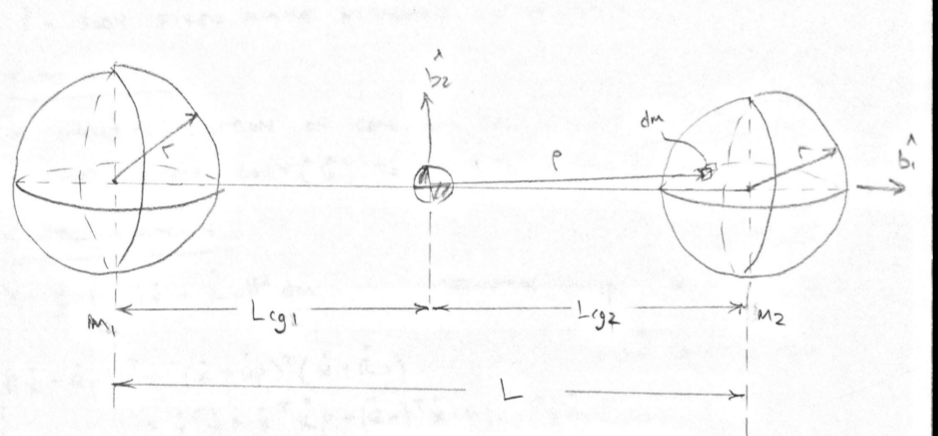
\includegraphics[width=\textwidth]{figures/dumbbell.png}
    \caption{Dumbbell Model of Rigid Spacecraft}
    \label{fig:dumbbell_sc}
\end{figure}
The spacecraft body fixed frame is centered at the center of mass of the vehicle.
The \( \vh{b}_1 \) is axis is aligned with the connecting rod while the \( \vh{b}_2, \vh{b}_3 \) axes span the plane orthogonal to the axis of symmetry of the dumbbell.
The distance from the center of mass to each mass is defined as
\begin{align}\label{eq:dumbbell_mass_distances}
    l_1 &= \frac{m_2}{m_1 + m_2} l, \\
    l_2 &= l - l_1.
\end{align}

\paragraph{Moment of Inertia Derivation}\label{sec:moment_of_inertia}
The inertia tensor/matrix of a rigid body is defined~\cite{greenwood1988} as
\begin{align}
    J_I = \int_{\mathcal{B}} \bracket{ \parenth{\vb{\rho}^T \vb{\rho} }I - \vb{\rho}\vb{\rho}^T} dm, 
\end{align}
where \( \vb{\rho} \in \R^3 \) is the position of a mass element \( dm \) in the body fixed frame of the spacecraft.
One can also use~\cref{eq:xTx} to define the inertia matrix in several other equivalent forms
\begin{align*}
    J_I &= \int_{\mathcal{B}} \bracket{ \parenth{\vb{\rho}^T \vb{\rho} }I - \vb{\rho}\vb{\rho}^T} dm, \\
        &= \int_{\mathcal{B}} \tr{\vb{\rho}\vb{\rho}^T} I - \vb{\rho}\vb{\rho}^T, \\
        &= \int_{\mathcal{B}} \vh{\rho}^T \vh{\rho} dm.
\end{align*}
The location of an infinitesimal mass element \( dm \) can be decomposed into
\begin{align}\label{eq:mass_element_position}
    \vc{\rho}_i = \vc{\zeta} + \vc{\eta}_i, 
\end{align}
where \( \vb{\zeta} \) is the location of the center of \( m_i \) in the spacecraft fixed frame while \( \vc{\eta} \) the position of \( dm \) with respect to the center of \( m_i \) and expressed in the spacecraft fixed frame.
\begin{figure}[htbp]
    \centering
    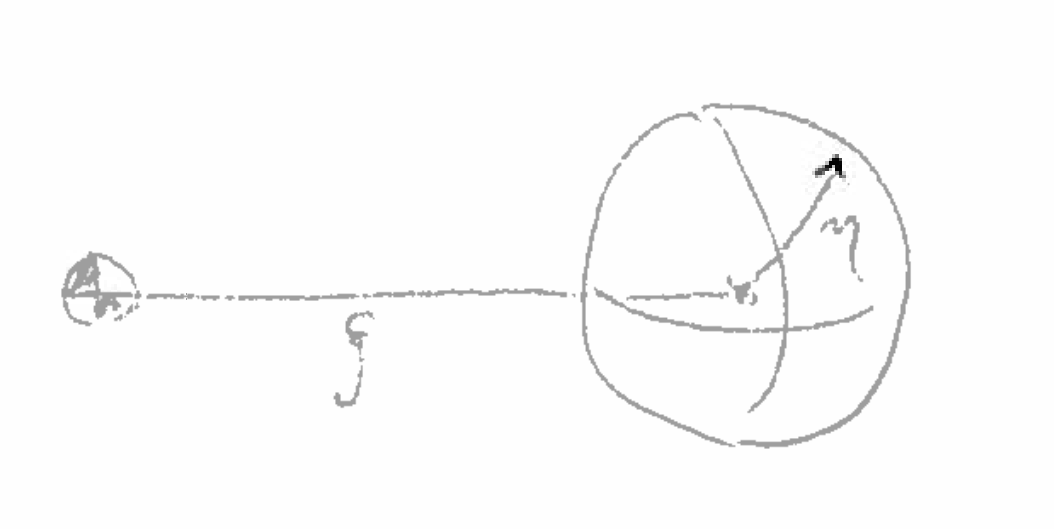
\includegraphics[width=\textwidth]{figures/dumbbell_pos_vector.png}
    \caption{Decomposition of mass element positon vector}
    \label{fig:dumbbell_moi_mass_element_position}
\end{figure}
Using~\cref{eq:mass_element_position} the moment of inertia can be expanded as
\begin{align*}
    J_I &= \sum_i^n \int_{\mathcal{B}_i} \parenth{\vc{\zeta}_i + \vb{\eta}_i}^T \parenth{\vc{\zeta}_i + \vc{\eta}_i } I  - \parenth{\vc{\zeta}_i + \vc{\eta}_i} \parenth{\vc{\zeta}_i + \vc{\eta}_i}^T dm .
\end{align*}
Further expansion leads to
\begin{align*}
    J_I = \sum_i^n \int_{\mathcal{B}_i} \parenth{\vc{\zeta}_i^T \vc{\zeta}_i}I - \vc{\zeta}_i \vc{\zeta}_i^T + \vc{\eta}_i^T \vc{\eta}_i I - \vc{\eta}_i \vc{\eta}_i^T dm, 
\end{align*}
since the cross terms include an integration over the constant density sphere goes to zero:
\begin{align*}
    \int_{\mathcal{B}_i} \vc{\eta}_i dm = 0 .
\end{align*}
The integration is now split into two components: an integration within each sphere, \( \vc{\eta}_i \) terms, and and integration involving the location of the sphere, \( \vc{\zeta}_i \) terms.
As a result, the final moment of inertia of a system of rigid spherical masses is 
\begin{align}\label{eq:dumbbell_moment_of_inertia}
    J_I = \sum_i J_i + m_i \parenth{\vc{\zeta}_i^T \vc{\zeta}_i I - \vc{\zeta}_i \vc{\zeta}_i^T} , 
\end{align}
where \( \vc{\zeta}_i \) is the position of \( m_i \) in the spacecraft fixed frame and the moment of inertia of each sphere is
\begin{align}\label{eq:sphere_moment_of_inertia}
    J_i = \begin{bmatrix} 
        \frac{2}{5} m_i r_i^2 & 0 & 0 \\
        0 & \frac{2}{5} m_i r_i^2 & 0 \\
        0 & 0 & \frac{2}{5} m_i r_i^2 
    \end{bmatrix}.
\end{align}
\Cref{eq:dumbbell_moment_of_inertia} is consitent with the well-known parallel-axis theorem~\cite{greenwood1988}.

%TODO Nonstandard moment of inertia matrix
\paragraph{Nonstandard Moment of Inertia Matrix}
The standard moment of inertia \( J \in \R^{3 \times 3} \) of a rigid body is given by
\begin{align}\label{eq:standard_moment_of_inertia}
    J = \int_{\mathcal{B}} \vh{\rho}^T \vh{\rho} dm 
    = \int_{\mathcal{B}}  
    \begin{bmatrix} 
        y^2 + z^2 & -xy & -zx \\
        -xy & z^2 + x^2 & -yz \\
        -zx & yz & x^2 + y^2
    \end{bmatrix} dm, 
\end{align}
where \( \vc{\rho} = \begin{bmatrix} x & y & z \end{bmatrix}\).
A nonstandard moment of inertia matrix \( J_d \in \R^{3 \times 3 } \) is defined as
\begin{align} \label{eq:nonstandard_moment_of_inertia}
    J_d = \int_{\mathcal{B}} \vc{\rho} \vc{\rho}^T dm = \int_{\mathcal{B}} 
    \begin{bmatrix}
        x^2 & xy & zx \\
        xy & y^2 & yz \\
        zx & yz & z^2
    \end{bmatrix} dm.
\end{align}
Using~\cref{eq:xTx} and the properties of the outer product, it can be shown that
\begin{subequations}\label{eq:moi_transformation}
    \begin{align}
        J &= \tr{J_d} I - J_d, \\
        J_d &= \frac{1}{2} \tr{J} I - J.
    \end{align}
\end{subequations}     
In addition, the following equation is also satisfied for any \( \vc{\Omega} \in \R^3 \)
\begin{align}\label{eq:moi_hat_prop}
    \parenth{J \vc{\Omega}}^\wedge = \vh{\Omega} J_d + J_d \vh{\Omega}.
\end{align}
\Cref{eq:moi_hat_prop} is easy to prove by substituting \( \vc{\Omega} = \begin{bmatrix} \Omega_1 & \Omega_2 & \Omega_3 \end{bmatrix} \) and expanding both sides of~\cref{eq:moi_hat_prop} to
\begin{align*}
    \begin{bmatrix}
        \parenth{J_{yy} + J_{zz}} \Omega_1 - J_{xy} \Omega_2 - J_{zx} \Omega_3 \\
        -J_{xy}\Omega_1 + \parenth{J_{zz} + J_{xx}} \Omega_2 - J_{yz}\Omega_3 \\
        -J_{zx}\Omega_1 - J_{yz}\Omega_2 + \parenth{J_{xx} + J_{yy}} \Omega_3
    \end{bmatrix}^\wedge,
\end{align*}
where \( J_{xy} = \int_{\mathcal{B}} xy dm \in \R \) and the other terms are defined simarily.

\subsection{Inertial Frame Equations of Motion}\label{sec:inertial_dumbbell_eoms}

\paragraph{Kinetic Energy of Dumbbell}\label{sec:inertial_kinetic_energy}
The kinetic energy of the spacecraft begins with the kinematics defined in~\cref{ssec:dumbbell_eoms_reference_frames} as
\begin{align}\label{eq:inertial_KE_1}
    T = \frac{1}{2} \int_{\mathcal{B}} \norm{ \dot{\vc{x}} + \dot{R} \vc{\rho}}^2 dm,
\end{align}
where \( \vc{\rho} \in \R^3 \) defines the position of the mass element \( dm \) in the body fixed frame of the spacecraft.
Expanding the quadratic term in~\cref{eq:inertial_KE_1} results in
\begin{align}\label{eq:inertial_KE_2}
T = \frac{1}{2} \int_{\mathcal{B}}  \norm{\dot{\vc{x}}}^2 + 2 \dot{\vc{x}}^T \dot{R} \vc{\rho} + \norm{\dot{R} \vc{\rho} }^2    dm .
\end{align}
\Cref{eq:inertial_KE_2} is further simplified by noting that
\begin{align*}
    \int_{\mathcal{B}} \vc{\rho} dm = 0,
\end{align*}
and from using the kinematics \( \dot{R} = \R \vh{\Omega} \) for \( \vc{\Omega} \in \R^3 \) 
\begin{align*}
    \norm{\dot{R} \vc{\rho} }^2 &= \vc{\rho}\dot{R}^T \dot{R} \vc{\rho} , \\
                                &=  \vc{\rho}^T \vh{\Omega}^T \vh{\Omega} \vc{\rho} , \\
                                &= \norm{ \vh{\Omega} \vc{\rho} }^2, 
\end{align*}
which results in the following expression for the kinetic energy
\begin{align}\label{eq:inertial_KE_3}
    T = \frac{1}{2} \int_{\mathcal{B}} \braces{ \norm{\dot{\vc{x}}}^2 + \norm{\vh{\Omega} \vc{\rho}}^2 } dm.
\end{align}
The second term \( \norm{\vh{\Omega}\vc{\rho}}^2 \) is simplified to
\begin{align}
    \norm{ \vh{\Omega}\vc{\rho} }^2 &= \parenth{ \vh{\Omega}\vc{\rho}}^T \parenth{\vh{\Omega}\vc{\rho}} , \\
                                    &= \tr{ \vh{\Omega} \vc{\rho} \vc{\rho}^T \vh{\Omega}^T }.
\end{align}
Applying this to~\cref{eq:inertial_KE_3} results in the final form of the kinetic energy as
\begin{align}\label{eq:inertial_kinetic_energy}
    T = \frac{1}{2} m \norm{\dot{\vc{x}}}^2 + \frac{1}{2} \tr{ \vh{\Omega}J_d \vh{\Omega^T } }, 
\end{align}
where we applied the non-standard moment of inertia defined in~\cref{eq:nonstandard_moment_of_inertia}.

\paragraph{Potential Energy of Dumbbell}
The potential energy of the dumbbell is a function of the asteroid potential model.
There are a number of possible models as shown in~\cref{sec:gravitational_models}.
For a rigid body composed of several spherical point masses, the total potential becomes
\begin{align}\label{eq:inertial_potential_energy}
    V(\vc{x}, R, R_A) = \sum_{i}^n - m_i U \parenth{R_A^T \parenth{\vc{x} + R \vc{\rho}_i}},
\end{align}
where \( \vc{x} \in \R^3\) is the position of the center of mass, \( R \in \SO\) is the rotation matrix which transforms vectors from the spacecraft frame to the inertial frame, and \( R_A \in \SO \) is the rotation matrix which transforms vectors from the asteroid frame to the inertial frame.

Using our kinematic variables we can define the kinetic and potential energy of the dumbbell using~\cref{eq:inertial_kinetic_energy,eq:inertial_potential_energy} as
\begin{subequations}\label{eq:dumbbell_kinetic_and_potential_energy}
\begin{align}
    T &= \frac{1}{2} m \norm{\dot{\vb{x}}}^2 + \frac{1}{2} \tr{\vh{\Omega} J_d \vh{\Omega}^T} , \label{eq:dumbbell_kinetic_energy}\\
    V( \vecbf{x}, R ) &=  - m_1 U \parenth{R_A^T \parenth{\vecbf{x} + R \vecbf{\rho}_1}} - m_2 U \parenth{R_A^T \parenth{\vecbf{x} + R \vecbf{\rho}_2}} , \label{eq:dumbbell_potential_energy}
\end{align}
\end{subequations}     
where we utilize the polyhedron potential is defined in~\cref{sec:polyhedron_potential}.
The position of each mass \(m_i\) of the dumbbell is defined in the dumbbell fixed frame by the vector \(\vc{\rho}_i\). 
With~\cref{eq:dumbbell_kinetic_and_potential_energy} one can then use Hamilton's principle to derive the equations of motion.
However, the first step is to determine the varations of \( T, V \).
These variations must be carefully constructed such that the variations of the configuration variables do not violate the nonlinear manifold.
The next step is to define the variations of the kinetic and potential energy to derive the equations of motion, which are given as
\begin{align} 
    \delta V &= -\sum_{i=1}^2  m_i \parenth{R_A \deriv{U}{\vb{z}_i} }^T \delta \vb{x} + m_i \hat{\vb{\eta}}\cdot \hat{\vb{\rho}_1} R^T R_A \deriv{U}{\vb{z}_i}, \label{eq:dumbbell_kinetic_energy_variation} \\
    \delta T &= \parenth{m_1 + m_2} \dot{\vecbf{x}}^T \delta \dot{\vb{x}} + \frac{1}{2} \tr{- \dot{\hat{\vb{\eta}}} S(J \vb{\Omega}) + \hat{\vb{\eta}} S(\hat{\vb{\Omega}} J \vb{\Omega})}. \label{eq:dumbbell_potential_energy_variation} ,
\end{align}
where \( \vc{z}_i = R_A^T \parenth{\vc{x} + R \vc{\rho}} \) and defines the position of \( m_i \) in the asteroid fixed frame.
The derivation of~\cref{eq:dumbbell_potential_energy_variation,eq:dumbbell_kinetic_energy_variation} is provided in~\cref{proof:inertial_dumbbell_eoms}.

Using the variations of the kinetic and potential energy we can derive the equations of motion of the dumbbell spacecraft about an asteroid using Hamilton's principle. 
Hamilton's principle then states that the variation of the action integral
\begin{align}
    \mathsf{G} = \int_{t_0}^{t_f} T(\dot{q}) - V(q) dt,
\end{align}
is stationary with fixed endpoints. 
Applying the calculus of variations and integration by parts results in the familiar Euler-Lagrange equations of motion.
Applying the Legendre transformation allows for the same dynamics to be expressed in an equivalent form as Hamilton's equations~\cite{lanczos1970}.
The equations of motion of a dumbbell spacecraft influenced by a polyhedron potential model are given as
\begin{align}
    \dot{\vb{x}} &= \vb{v}, \label{eq:position_kinematics}\\
    \parenth{m_1 + m_2} \dot{\vecbf{v}} &= m_1 R_A \deriv{U}{\vecbf{z}_1} + m_2 R_A \deriv{U}{\vecbf{z}_2} + \vecbf{u}_f, \label{eq:translational_dynamics}\\
    \dot{R} &= R S(\vb{\Omega}) , \label{eq:attitude_kinematics}\\
    J \dot{\vecbf{\Omega}} + \vecbf{\Omega} \times J \vecbf{\Omega} &= \vecbf{M}_1 + \vecbf{M}_2 + \vecbf{u}_m. \label{eq:attitude_dynamics}
\end{align}
The vectors \( \vecbf{z}_1 \) and \( \vecbf{z}_2\) define the position of the dumbbell masses as represented in the asteroid fixed frame and are defined as
\begin{align}
    \vecbf{z}_1 &= R_A^T \parenth{\vecbf{x} + R \vecbf{\rho}_1} , \\
    \vecbf{z}_2 &= R_A^T \parenth{\vecbf{x} + R \vecbf{\rho}_2}, 
\end{align}
where \( \vb{\rho}_i \) defines the position of each mass in the spacecraft fixed body frame.
The gravitational moment on the dumbbell \( \vecbf{M}_i\) is defined as
\begin{align}
    \vecbf{M}_i = m_i \parenth{S(R_A^T \vb{\rho}_i) R^T \deriv{U}{\vb{z}_i}}.
\end{align}
The control inputs to the spacecraft are defined by \( \vb{u}_f, \vb{u}_m \) which define the control force represented in the inertial frame and the control moment represented in the spacecraft frame, respectively. 

\subsection{Asteroid Frame Equations of Motion}


\section{Gravitational Models around Small-Bodies}\label{sec:gravitational_models}
Due to the irregular shape of small-bodies, the gravitational field around these bodies is equally irregular.
Furthermore, the relative size of the spacecraft in comparison with the orbital radius and small-body creates a much larger coupling between the translational and rotational states of the spacecraft.
In addition, spacecraft will tend to operate in very close proximity to the surface.
As a result, accurate computation of the gravitational field around these irregular bodies is critical to safe and effective operations.
The classic approach to determining the gravitational force is to apply Newton's law of Universal gravitation.
The force due to gravity between two point masses is defined as
\begin{align}\label{eq:newton_universal_gravitation}
    \vb{F}_g =  - G \frac{m_1 m_2}{r^2} \frac{\vb{r}}{r},
\end{align}
where \( G \) is the universal gravitational constant, \( \vb{r} \) is the relative position vector between the points of mass \( m_1, m_2\), respectively.

\begin{figure}
    \centering
    \includegraphics[width=\textwidth]{example-image-golden}
    \caption{Newton's Law of Unviversal Gravitation~\label{fig:universal_gravity}}
\end{figure}

This gravitational model is defined if point masses or bodies which can be modeled as point masses, such as spherically symmetric planets.
However, it is not possible to model an irregular asteroid, or an orbiting spacecraft, as point masses.
Instead, one must treat both bodies as extended objects and compute the gravitational force from the potential function as an integral over the entire body, \( \mathcal{B}\),
\begin{align}\label{eq:volume_integral_potential}
\vb{F}_g ( \vb{r}) = \nabla U = G \int_{\mathcal{B}} \frac{1}{\norm{\vb{r} - \vb{\rho} }} dm (\vb{\rho}),
\end{align}
where \( \vb{r} \) is the position of the field point, \( \vb{\rho} \) is the position of the differential mass element of the body and \( \nabla U \) is defined as the gradient of \( U \) with respect to the standard cartesian basis vectors
\begin{align*}
    \nabla = \deriv{}{x} \hat{\vb{i}} + \deriv{}{y} \hat{\vb{j}} + \deriv{}{z} \hat{\vb{k}}.
\end{align*}

The first approach, sometimes termed the \textit{mass-concentration}, or \textit{mascon} method, approximates the integral using an infinite sum of point masses \( m_i\) located at \( \vb{r}_i \).
The potential on our object of interest then becomes the summation of the potential caused by each mass \( m_i \) as shown in~\cref{eq:mass_con_potential}.
\begin{align}\label{eq:mass_con_potential}
    U = G \sum_{i=0}^{\infty} \frac{m_i}{\norm{\vb{r} - \vb{\rho}_i}}
\end{align}
The method distributes a colleciton of point masses uniformly throughout the body such that the total mass is equal to the body.
While conceptually simple, and relatively straight forward to numerically implement, the mascon approach has several drawbacks~\cite{scheeres2012a}.
First, the mascon approach does not provide any method to determine if the object of interest is inside or outside of the body.
As a result, any numerical simulation making use of the mascon approach will require a secondary operation to determine if the spacecraft has collided with the surface.
Additionaly, it has been shown that the mascon approach is more computationaly demanding than other methods, namely the spherical harmonic or polyhedron potential method~\cite{werner1996}.
Finally, while the mascon method will provide the true gravity field in the limit as the number of invidual point masses becomes large, there are significant errors in the direction of the force vector~\cite{werner1996}.

It can be shown that the gravitational potential will satisfy Laplace's equation outside of the body
\begin{align}
    \nabla^2 U = 0
\end{align}
and Poisson's equation inside of the body
\begin{align}
    \nabla^2 U = - 4 \pi G \sigma
\end{align}
where \( \sigma \) is the local density of the body.
Laplace's equation can be solved using a seperation of variables in terms of spherical coordinates~\cite{scheeres2012a}.
The transformation between cartesian, \( \vb{r} = x \hat{\vb{x}} + y \hat{\vb{y}} + z \hat{\vb{z}}\),  and spherical coordinates, is given by
\begin{subequations}
    \begin{align*}
        r &= \sqrt{x^2 + y^2 + z^2}, \\
        \sin \phi &= \frac{z}{r}, \\
        \tan \lambda &= \frac{y}{x},
    \end{align*}
\end{subequations}
where \( \phi \) is the latitude and \( \lambda\) is the longitude.
One can then follow a standard derivation~\cite{vallado2007} to arrive at a general form of the spherical harmonic potential model:
\begin{align}\label{eq:spherical_harmonic}
    U = \frac{\mu}{r} \sum_{l=0}^\infty \sum_{m=0}^l \parenth{\frac{r_o}{r}}^n P_{l, m}(\sin \phi) \braces{ C_{lm} \cos(m \lambda) + S_{lm} \sin(m \lambda)},
\end{align}
where \( \mu = G M \) is the gravitational parameter of the body, \( r_o\) is a normalizing radius, which is typically chosen as the mean or maximum radius of the attracting body.
The term \( P_{l, m} \) are the associated Legendre functions while \( C_{lm}\) and \( S_{lm}\) are called the spherical harmonic coefficients or Stoke's coefficients. 
The Legendre functions are given in closed form by~\cite{scheeres2012}
\begin{subequations}
\begin{align}
    P_{l, m} \parenth{ \sin \delta} &= \cos^m \phi \sum_{i = 0}^{\text{int}\bracket{l - \frac{m}{2}}} T_{lmi} \sin^{l - m - 2i} \phi ,  \\
T_{lmi} &= \frac{\parenth{-1}^i\parenth{2l - 2i}!}{2^l i! \parenth{l - i}!\parenth{l - m- 2i}!}.
\end{align}
\end{subequations}
where \( \text{int}\bracket{x}\) defines the integer portion of \( x \).
Defining the spherical harmonic coefficients, namely \( C_{lm}, S_{lm}\), is equivalent to defining the mass distribution of the body.
The spherical harmonic coefficients have been determined for many planetary bodies, such as the Earth, to a very high fidelity~\cite{vallado2007,pavlis2012}.

% TODO Continue with the drawbacks of spherical harmonic
The spherical harmonic gravity model is not applicable in all situations.
A implicit assumption of the spherical harmonic expansion are that the series converge to the true gravitational field.
It can be shown that the expansion will diverge when applied to a point within the maximum circumscribing sphere of the body~\cite{scheeres2012a}.
A typical remedy is to derive two different expansions, the first:
\begin{align}
    U = \frac{1}{V} \int_{\mathcal{B}} \parenth{ \frac{\rho}{r}}^i P_{i0} \parenth{ \frac{\vb{r} \cdot \vb{\rho}}{ r \rho}} dV, 
\end{align}
is only valid when \( \norm{\rho} < r \) and is not defined at \( \norm{\vb{\rho}} = r\).
A second expansion can be derived for the case \(\norm{\vb{\rho}} > r \) as
\begin{align}
    U = \frac{1}{V} \int_{\mathcal{B}} \parenth{ \frac{r}{\rho}}^i P_{i0} \parenth{ \frac{\vb{r} \cdot \vb{\rho}}{ r \rho}} dV. 
\end{align}
If a finite density is assumed, then the gravitational field will vanish at \( \norm{\vb{\rho}} = r \).
As a result of this discontinuity, the expansion coefficients become a function of the radius of the body and must be recomputed as the body changes.
These limitations mean that in practice the spherical harmonic expansion model cannot be used for the gravity model when operating around an irregular body.
The divergence of the expansion causes the gravitational field to become meaningless when close to the surface and make the use of the spherical harmonic model worthless for dynamic computations.

% TODO Add picture of biroullion sphere
% TODO Add glossary entry for biroullion sphere
% TODO Show picture of point masses and newton's law and add near the equation
% TODO Add picture of MASCON model (many point masses)

An alternative approach is based on using a specified shape of the body to determine a closed form solution to the gravitational potential.
Each of these methods are based on a known shape of the body and a strong assumption on the density variation, frequently assuming a homegenous body with constant density.
The simplest solution is based on a spherical body with a radially-varying density distribution.
This type of model is best applicable for centrobaric bodies, such as the Earth and many planetary bodies.
% TODO Write down the spherical potential for a radially varying distribution from AAE532
The solutions for the constant density ellipsoid and constant density polyhedron are more useful for operations near small irregular bodies.
These methods provide exact, closed-form solutions which are valid up to the surface of the body and have been used in the majority of research near the surface of small bodies.
Here we present the ellipsoid and polyhedron potential models which are commonly used heavily used in research around small bodies.

\subsection{Constant Density Ellipsoid}\label{sec:constant_density_ellipsoid}

% TODO Need to add citations for these statements
The ellipsoid gravitational model assumes that the small body is accurately represented by a constant density ellipsoid.
This strong assumption is appropriate for many bodies as they are relatively close to ellipsoidal in shape.
Furthermore, many asteroids are also well represented with a constant density. 
In addition, based on ground measurements alone it is frequently not possible to arrive at a more accurate shape beyond that of a triaxial ellipsoid.
The triaxial ellipsoid has semi-major axes \( \gamma \leq \beta \leq \alpha\) and the surface of the body is defined by the implicit equation
\begin{align}
    \parenth{\frac{x}{\alpha}}^2 + \parenth{\frac{y}{\beta}}^2 + \parenth{\frac{z}{\gamma}}^2 \leq 1 . 
\end{align}
% TODO Draw a picture of ellipsoid with teh axes labeled
\begin{figure}
    \centering
    \includegraphics[width=\textwidth]{example-image-golden}
    \caption[Triaxial Ellipsoid]{Constant Density Tri-Axial Ellipsoid Model~\label{fig:triaxial_ellipsoid}}
\end{figure}
Using this model, the gravitational potential outside the body is given by
\begin{subequations}
\begin{align}
    U (\vb{r}) &= - \frac{3 \mu}{4} \int_{\lambda{\vb{r}}}^{\infty} \frac{\phi ( \vb{r},  u) }{ \Delta(u)} du, \\
    \phi(\vb{r}, u) &= \frac{x^2}{\alpha^2 + u} + \frac{y^2}{\beta^2 + u} + \frac{z^2}{\gamma^2 + u} - 1 , \\
    \Delta(u) &= \sqrt{\parenth{\alpha^2 + u} \parenth{\beta^2 + u} \parenth{\gamma^2 + u}},
\end{align}
where \( \lambda(\vb{r}) \) is defined by \( \phi(\vb{r}, \lambda) = 0 \).
The position vector should be transformed into the principle axis frame, such that the \( \hat{\vb{x}} \) axis is aligned along the long axis \( \alpha \), \( \hat{\vb{y}} \) is aligned with the intermediate axis \( \beta \), and \( \hat{\vb{z}} \) is aligned along the short axis \( \gamma \).
A straightforward application of Leibniz's rule allows one to compute the Jacobian and Hessian of \( U \)~\cite{scheeres2012a}.
\end{subequations}  

The constant density ellipsoid model provides a closed form solution for the gravitational potential but suffers from a number of disadvantages.
It is based on a specific body shape, namely the triaxial ellipsoid, and is not applicable for bodies that have a different shape.
Approximating the shape of many small bodies as triaxial ellipsoids is appropriate for many first order dynamical simulations and analysis.
Insight into the dynamic environment~\cite{guelman2014}, periodic orbits~\cite{hu2002}, equilibrium points~\cite{scheeres1994}, or surface dynamics~\cite{furfaro2013} are all greatly simplified with use of the ellipsoid shape approximation.
However, once additional data is received, such as improved ground imaging or in-situ measurements from a spacecraft, the shape model of the small body will become more accurate and cause it to diverge from the ellipsoid assumption.
At this point, the dynamic model is no longer valid and must be modified for use with the updated shape data.
In the case of an operational mission, this may require extensive redevelopment of core flight software and the associated testing to ensure it is functioning properly. 
Furthermore, the model is defined in terms of continuous integrals which must be numerically evaluated using methods of Carlson's elliptic integrals.
Due to these reasons, we instead model the gravitational potential using the polyhedron potential model which alleviates many of these issues.

\subsection{Polyhedron Potential Model}\label{sec:polyhedron_potential}

% TODO Intro to the potnetial model. Cite some papers. Discuss the benefits
Robert Werner developed the polyhedron potential model in a series of papers in the mid-1990s~\cite{werner1994,werner1996,werner1997}.
The method provides a closed form solution for the gravitational potential about any arbitrary constant density polyhedron.
While the solution is closed form, the implementation requires efficient software to compute the potential as it is dependent on a summation over all faces and edges of the polyhedron.
There is no requirement on the polyhedron shape and it can incorporate craters, ridges, or even holes through the small body.
Furthermore, the accuracy of the model is solely dependent on the fidelity of the shape in representing the true body and the constant density assumption.
For bodies with varying density, it is possible to augument the polyhedron potential model to account for the density variations~\cite{scheeres2000a}.
This approach alleviates the divergence issue of the spherical harmonic model and is applicable for all points on or above the surface and is ideal for general operations around small bodies.
The polyhedron potential model has become the defacto standard for small body missions and has been used operationally.
In this section we summarize the polyhedron potential model based on the derivations of Werner.
We additionally present some of the implementation details in our model and the adaptions for use with the \texttt{Surface\_mesh} data structure presented  in~\cref{sec:polyhedron_data_structures}.

% TODO Add a link to the section that talks about polyhedrons
This model is composed of a polyhedron, which is a three-dimensional solid body, that is defined by a series of vectors in the asteroid fixed frame.
The vectors define vertices in the asteroid fixed frame and combinations of these vertices then define planar faces which compose the surface of the asteroid.
Additionally, we assume that each face is a triangle composed of three vertices and three edges.
As a result, only two faces meet at each edge while three faces meet at each vertex.
Only the body-fixed vectors, and their associated topology, is required to define the exterior gravitational model.

% TODO Need a picture of the edges/faces/halfedges
Consider three vectors \( \vecbf{v}_1, \vecbf{v}_2, \vecbf{v}_3 \in \R^{3 \times 1} \), assumed to be ordered in a counterclockwise direction about an outward facing normal vector, which define a face.
It is easy to define the three halfedges of each face as
\begin{align}\label{eq:edges}
    \vecbf{h}_{i} = \vecbf{v}_{i+1} - \vecbf{v}_i \in \R^{3 \times 1 },
\end{align}
where the index \( i \in \parenth{1,2,3} \) is used to permute all vertices of each face.
Each halfedge has an opposing or inverse which is a member of the adjacent face and orientated in the opposite direction.
We can also define the outward normal vector to each face \( f \) as
\begin{align}\label{eq:face_normal}
    \hat{\vecbf{n}}_f &= \parenth{\vb{h}_2} \times \parenth{\vb{h}_1} \in \R^{3 \times 1},
\end{align}
and the outward facing normal vector to each halfedge as
\begin{align}\label{eq:edge_normal}
    \hat{\vecbf{n}}_{i}^f &= - \parenth{\vb{h}_i} \times \hat{\vecbf{n}}_f \in \R^{3 \times 1}.
\end{align}
For each face, we define the face dyad \( \vecbf{F}_f \) as
\begin{align}\label{eq:face_dyad}
    \vecbf{F}_f &= \hat{\vecbf{n}}_f \hat{\vecbf{n}}_f \in \R^{3 \times 3}.
\end{align}
Each edge is a member of two faces and has an outward pointing edge normal vector, given in~\cref{eq:edge_normal}, perpendicular to both the edge and the face normal.
For the edge connecting the vectors \( \vecbf{v}_1 \) and \( \vecbf{v}_2 \), which are shared between the faces \(A\) and \( B\), the per edge dyad is given by
\begin{align}\label{eq:edge_dyad}
    \vecbf{E}_{12} = \hat{\vecbf{n}}_A \hat{\vecbf{n}}_{12}^A + \hat{\vecbf{n}}_B \hat{\vecbf{n}}_{21}^B \in \R^{3 \times 3}.
\end{align}
The edge dyad \( \vecbf{E}_e  \), is defined for each edge and is a function of the two adjacent faces meeting at that edge.
The face dyad \( \vecbf{F}_f \), is defined for each face and is a function of the face normal vectors.

Let \( \vecbf{r}_i \in \R^{3 \times 1} \) be the vector from the spacecraft to the vertex \( \vecbf{v}_i \) and it's length is given by \( r_i = \norm{\vecbf{r}_i} \in \R^{1} \).
The per-edge factor \( L_e \in \R^{1}\), for the edge connecting vertices \( \vecbf{v}_i \) and \( \vecbf{v}_j \), with a constant length \( e_{ij} = \norm{\vecbf{e}_{ij}} \in \R^1\) is
\begin{align}\label{eq:edge_factor}
    L_e &= \ln \frac{r_i + r_j + e_{ij}}{r_i + r_j - e_{ij}}.
\end{align}
For the face defined by the vertices \( \vecbf{v}_i, \vecbf{v}_j, \vecbf{v}_k \) the per-face factor \( \omega_f \in \R^{1} \) is
\begin{align}\label{eq:face_factor}
    \omega_f &= 2 \arctan \frac{\vecbf{r}_i \cdot \vecbf{r}_j \times \vecbf{r}_k}{r_i r_j r_k + r_i \parenth{\vecbf{r}_j \cdot \vecbf{r}_k} + r_j \parenth{\vecbf{r}_k \cdot \vecbf{r}_i} + r_k \parenth{\vecbf{r}_i \cdot \vecbf{r}_j}}.
\end{align}
The gravitational potential due to a constant density polyhedron is then given as
\begin{align}\label{eq:potential}
    U(\vecbf{r}) &= \frac{1}{2} G \sigma \sum_{e \in \text{edges}} \vecbf{r}_e \cdot \vecbf{E}_e \cdot \vecbf{r}_e \cdot L_e - \frac{1}{2}G \sigma \sum_{f \in \text{faces}} \vecbf{r}_f \cdot \vecbf{F}_f \cdot \vecbf{r}_f \cdot \omega_f \in \R^1,
\end{align}
where \( \vecbf{r}_e\) and \(\vecbf{r}_f \) are the vectors from the spacecraft to any point on the respective edge or face, \( G\) is the universal gravitational constant, and \( \sigma \) is the constant density of the asteroid.
Furthermore, we can use these definitions to define the attraction, gravity gradient matrix, and Laplacian as
\begin{align}
    \nabla U ( \vecbf{r} ) &= -G \sigma \sum_{e \in \text{edges}} \vecbf{E}_e \cdot \vecbf{r}_e \cdot L_e + G \sigma \sum_{f \in \text{faces}} \vecbf{F}_f \cdot \vecbf{r}_f \cdot \omega_f \in \R^{3 \times 1} , \label{eq:attraction}\\
    \nabla \nabla U ( \vecbf{r} ) &= G \sigma \sum_{e \in \text{edges}} \vecbf{E}_e  \cdot L_e - G \sigma \sum_{f \in \text{faces}} \vecbf{F}_f \cdot \omega_f \in \R^{3 \times 3}, \label{eq:gradient_matrix}\\
    \nabla^2 U &= -G \sigma \sum_{f \in \text{faces}}  \omega_f \in \R^1.\label{eq:laplacian}
\end{align}

One interesting thing to note is that both~\cref{eq:face_dyad,eq:edge_dyad} can be precomputed without knowledge of the position of the satellite.
They are both solely functions of the vertices and edges of the polyhedral shape model and are computed once and stored.
Once a position vector \( \vecbf{r} \) is defined, the scalars given in~\cref{eq:edge_factor,eq:face_factor} can be computed for each face and edge.
Finally,~\cref{eq:potential} is used to compute the gravitational potential at any point \( \vb{r} \) in the asteroid fixed frame.
The Laplacian, defined in~\cref{eq:laplacian}, gives a simple method to determine if the spacecraft has collided with the body~\cite{werner1996}. 
For all points outside the body~\cref{eq:laplacian} is equal to zero and becomes \( 4 \pi \) when inside the body.

The polyhedron potential model is defined as a summation over the faces and edges as shown in~\cref{eq:potential,eq:attraction,eq:gradient_matrix}.
Some terms, such as~\cref{eq:edge_factor,eq:face_factor}, are computed based on data within each face or edge, respectively.
While other terms, such as~\cref{eq:face_dyad,eq:edge_dyad}, require the topology of the polyhedron as they are dependent on the specific neighboring face or edge.
As a result, an efficient procedure is required to determine, store, and update the connectivity of the polyhedron. 
The standard method to describe the small body shape is in the OBJ format~\cite{neese2004}, which only defines the vertices and faces as described in~\cref{sec:polyhedron_data_structures}.
Therefore, the additional connectivity information, such as the adjacent faces, opposite halfedges, or unique edges, must be stored in an additional data structure which is accurately traversed.
For these reasons, the polyhedron potential model is implemented using a halfedge data structure, as implemented in the \texttt{Surface\_mesh} class of CGAL and described in~\cref{sec:halfedge_data_structure}.


 

